\section{Evaluation Lösungsprinzipien}

Aus der vorhergehenden Technologierecherche wird pro Studiengang ein Morphologischer Kasten erstellt. Dieser wird befüllt mit den Teilfunktionen und den recherchierten Technologien. Damit werden die Lösungsprinzipien evaluiert und verschiedene Varianten werden gefunden. Ein Überblick ueber alle Morphologischen Kasten befindet sich im Anhang \ref{Morphologischer Kasten}.

\subsection{Maschinentechnik Morphologischer Kasten}

PLACEHOLDER

\subsection{Elektrotechnik Morphologischer Kasten}

PLACEHOLDER

\subsection{Informatik Morphologischer Kasten}

Aus der Technologierecherche wurde folgender Morphologischer Kasten mit drei Varianten für die Informatik Teilfunktionen erstellt.

\begin{figure}[H]
\centering
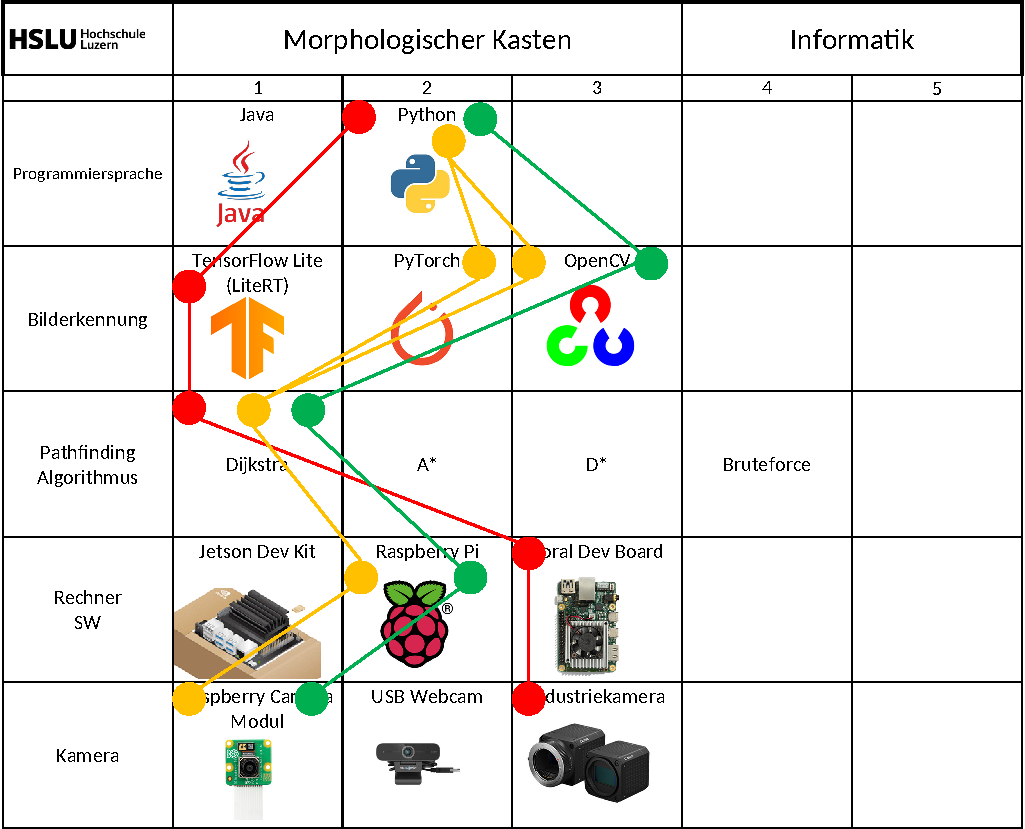
\includegraphics[width=\textwidth]{assets/MK_Informatik.pdf}
\caption{Morphologischer Kasten: Informatik}
\label{fig:mk-informatik}
\end{figure}

Es gibt nun drei Lösungskombinationen, die in einem nächsten Schritt evaluiert werden.

\begin{enumerate}
    \item Python verwendet LiteRT, um mit AI die Umgebung zu erkennen und Dijkstra, um den Weg zu berechnen. Das Ganze rechnet auf einem Coral Dev Board und fotografiert den Graphen mit einer Industriekamera.
    \item Python verwendet eine Mischung aus PyTorch und OpenCV, um AI und reine Bilderkennung zu verwenden. Dijkstra berechnet den Weg. Das Ganze rechnet auf einem Raspberry Pi mit einer Raspberry Camera angeschlossen.
    \item  Python verwenden nur OpenCV zur Bilderkennung und berechnet mit Dijkstra den Weg, es rechnet auf einem Raspberry Pi mit einer Raspberry Camera.
\end{enumerate}

Bei den drei Varianten fällt auf, dass alle Python und den Wegfindealgorithmus Dijkstra verwenden würden. Python wurde immer gewählt, da Bilderkennung und Machine Learning sehr gut mit Python harmonisieren. Viele Libraries, inklusive dieser, die hier ersichtlich sind, sind kompatibel mit Python. Dijkstra wurde immer gewählt, weil dieser Algorithmus simpel und robust ist und die Geschwindigkeit vernachlässigbar ist. Da es im Graphen nur 8 Knoten gib, wird die Berechnung bei jedem Algorithmus schnell sein.

\subsection{Simulator Morphologischer Kasten}


Aus der Technologierecherche wurde folgender Morphologischer Kasten für die Teilfunktonen des Simulators erstellt. Es gibt drei Varianten, die in Frage kommen.

\begin{figure}[H]
\centering
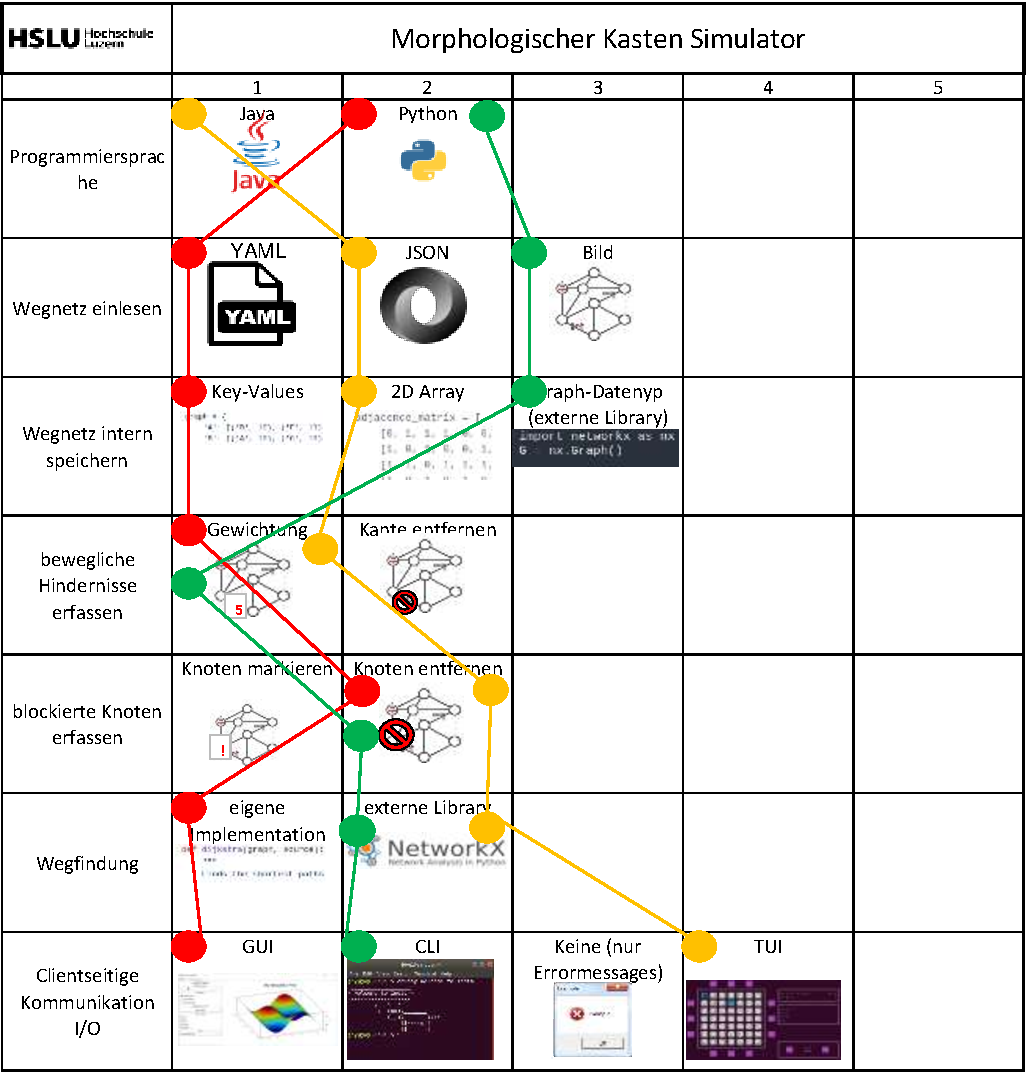
\includegraphics[width=\textwidth]{assets/MK_Simulator.pdf}
\caption{Morphologischer Kasten: Simulator}
\label{fig:mk-simulator}
\end{figure}

Die folgenden drei Lösungskombinationen, werden im nächsten Schritt evaluiert.

\begin{enumerate}
    \item 
\end{enumerate}
Kante entfernen nicht, weil gibt ev keinen Weg mehr, zu risky: Robustheit

Knoten nur markieren nicht noetig, bringt keinen Vorteil


\newpage
\section{Auswahl Lösungskombinationen}

Zur Auswahl der passendsten Lösungskombination wird pro Teilbereich eine Nutzwertanalyse durchgeführt. Die Kriterien und deren Gewichtung sind individuell pro Teilbereich, damit sie ideal passen.

\subsection{Maschinentechnik Nutzwertanalyse}

PLACEHOLDER

\subsection{Elektrotechnik Nutzwertanalyse}

PLACEHOLDER

\subsection{Informatik Nutzwertanalyse}

PLACEHOLDER

\subsection{Simulator Nutzwertanalyse}

PLACEHOLDER

Schnelligkeit vernachlaessigbar weil: nur 8 Knoten und weil macht sehr wenig aus, viel wichtiger ist Lightweight, da nur 1 Raspi in Realitaet und wollen moeglichst realitaetsgetreu das machen

\newpage
\section{Gesamtkonzept}

Aus den morphologischen Kasten und den Nutzwertanalysen wurde folgendes Gesamtkonzept ermittelt. 

